\subsection[Declarative vs Imperative]{Declarative vs Imperative Programming}

\frame{\tableofcontents[currentsection, currentsubsection]}

\begin{frame}{Declarative vs imperative programming}
	\hhl{Declarative programming}:
	\begin{itemize}
		\item Programm describes \hl{logic} rather than \hl{control flow}
		\item Program describes \hl{\enquote{what}} rather than \hl{\enquote{how}}
		%\item Focus on \hl{description} rather than \hl{implementation}
		\item Aims for correspondence with mathematic logic
		\item \hl{FP} is usually considered a subcategory
	\end{itemize}
	
	\medskip
	Opposite: \hhl{imperative programming}:
	\begin{itemize}
		\item Algorithms as a sequence of steps
		\item Often used synonymously: \hhl{procedural programming} \srem{(emphasizing the concept of using procedure calls (functions) to structure the program in a modular fashion)}
		\item \hl{OOP} is usually considered a subcategory
	\end{itemize}
\end{frame}

\begin{frame}{Examples}
	Picture book examples:
	\begin{itemize}
		\item \proglang{SQL} \srem{(Structured Query Language -- language to interact with databases $\lra$ \mauthor{Emil Kleszcz})}:
		%
		\begin{center}
			\mintinline{SQL}{SELECT * FROM Customers WHERE Country='Mexico';}
		\end{center}
		\item \hhl{Markup languages}, like \proglang{HTML}, \proglang{CSS} \srem{(Cascading Style Sheets -- language to describe styling of e.g. HTML pages)}, \dots
		%
		\begin{center}
			\mintinline{HTML}{<h1 style="color:blue;">This is a Blue Heading</h1>
			}
		\end{center}
		\item Strict functional programming languages like \proglang{Haskell}
		\item \dots
\end{itemize}
\end{frame}

\begin{frame}{Referential transparency}
	% https://stackoverflow.com/questions/210835/what-is-referential-transparency
	
	
\end{frame}
%
\begin{frame}{A broader definition...}
	Using powerful backends, your source code starts to look very declarative
\end{frame}
%
%
\begin{frame}{Powerful backends I}
	Comparison of code fragments using \texttt{numpy}, \texttt{scipy}: Plain python (loops etc.), numpy (declarative), scipy (our problem is already solved)
\end{frame}
%
%
\begin{frame}{Powerful backends II}
	\begin{itemize}
		\item \texttt{pandas} \srem{(\proglang{python} package to describe operations on tables)} can be viewed as a \enquote{declarative language} $\lra$ have a more sophisticated backend handle all operations $\lra$ \texttt{modin pandas}
		
		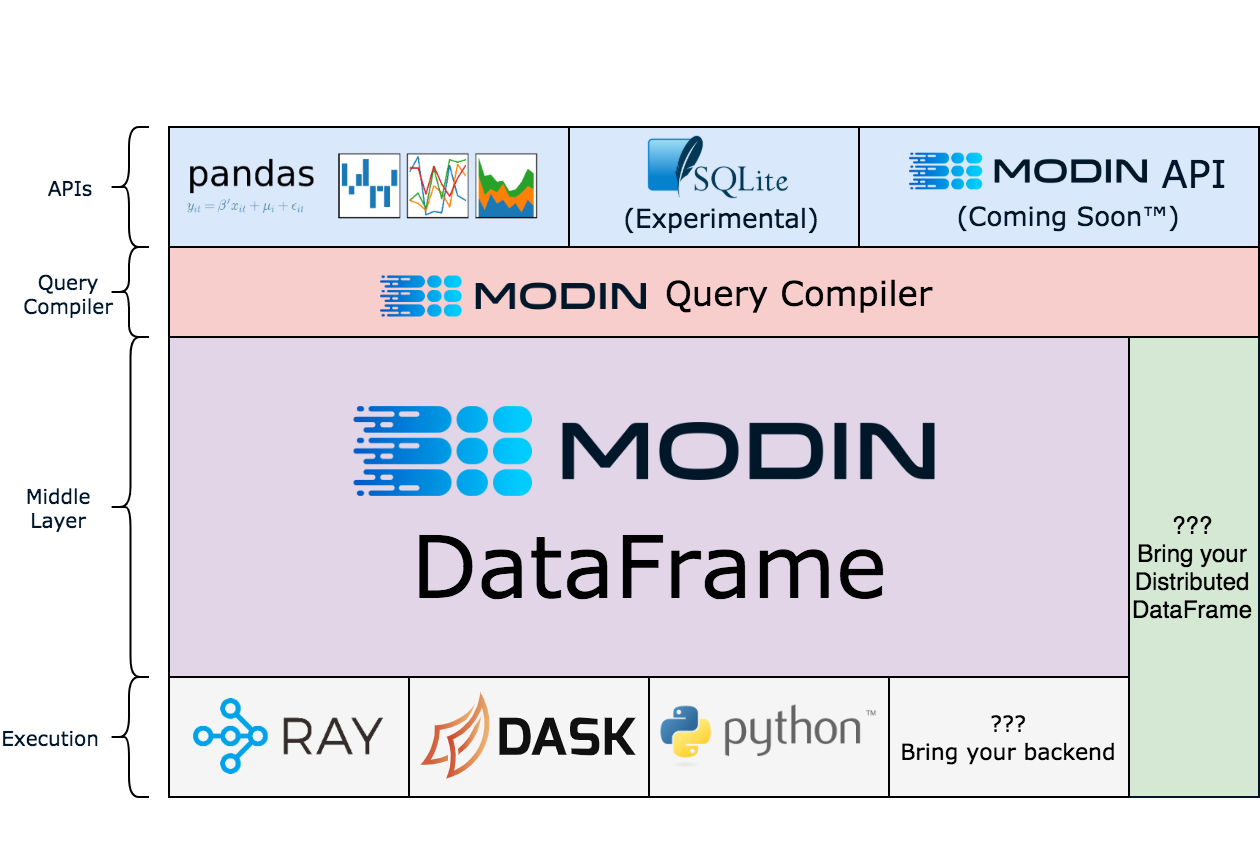
\includegraphics[width=8cm, trim=0cm 2.5cm 0cm 2.5cm, clip]{figures/paradigms/dp/modin_architecture.png}
		%
		\item \proglang{ROOT} can also do dataframes: \texttt{RDataFrame}
	\end{itemize}
\end{frame}
%
\begin{frame}{Powerful backends III}
	Many new things coming specifically for HEP, e.g. LINQToROOT
\end{frame}